% Created by tikzDevice version 0.12.6 on 2024-06-11 19:57:13
% !TEX encoding = UTF-8 Unicode
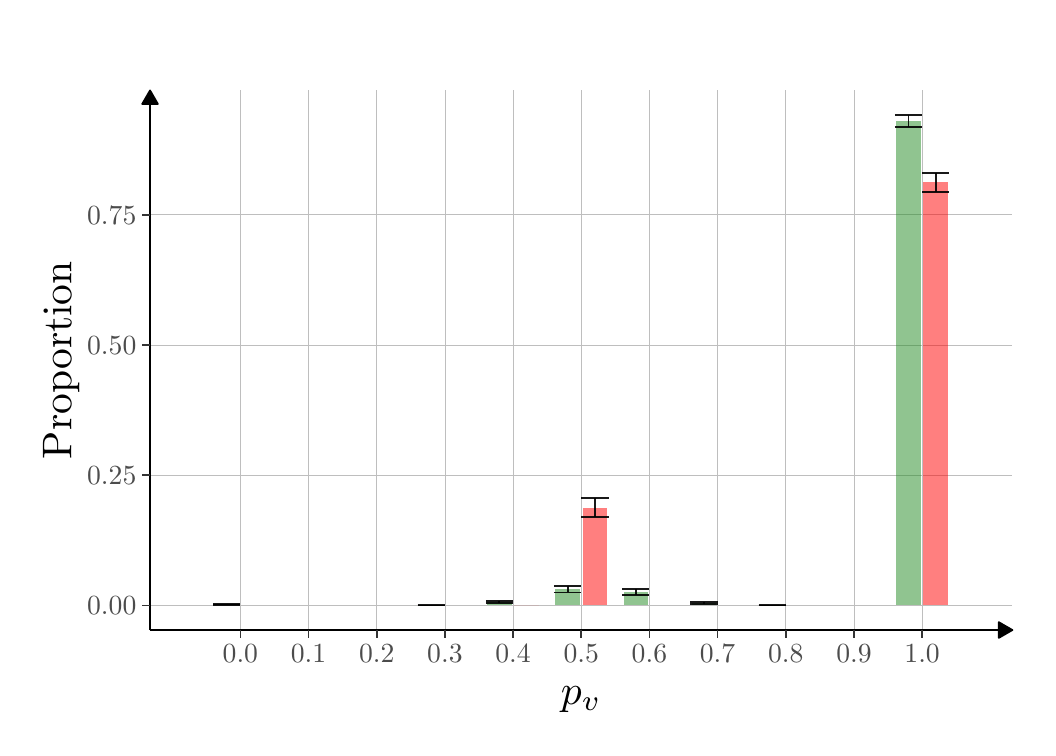
\begin{tikzpicture}[x=1pt,y=1pt]
\definecolor{fillColor}{RGB}{255,255,255}
\path[use as bounding box,fill=fillColor,fill opacity=0.00] (0,0) rectangle (361.35,252.94);
\begin{scope}
\path[clip] (  0.00,  0.00) rectangle (361.35,252.94);
\definecolor{drawColor}{RGB}{255,255,255}
\definecolor{fillColor}{RGB}{255,255,255}

\path[draw=drawColor,line width= 0.6pt,line join=round,line cap=round,fill=fillColor] (  0.00,  0.00) rectangle (361.35,252.94);
\end{scope}
\begin{scope}
\path[clip] ( 44.22, 35.28) rectangle (355.85,230.29);
\definecolor{fillColor}{RGB}{255,255,255}

\path[fill=fillColor] ( 44.22, 35.28) rectangle (355.85,230.29);
\definecolor{drawColor}{RGB}{255,255,255}

\path[draw=drawColor,line width= 0.3pt,line join=round] ( 44.22, 67.71) --
	(355.85, 67.71);

\path[draw=drawColor,line width= 0.3pt,line join=round] ( 44.22,114.75) --
	(355.85,114.75);

\path[draw=drawColor,line width= 0.3pt,line join=round] ( 44.22,161.79) --
	(355.85,161.79);

\path[draw=drawColor,line width= 0.3pt,line join=round] ( 44.22,208.82) --
	(355.85,208.82);

\path[draw=drawColor,line width= 0.3pt,line join=round] ( 52.23, 35.28) --
	( 52.23,230.29);

\path[draw=drawColor,line width= 0.3pt,line join=round] ( 64.54, 35.28) --
	( 64.54,230.29);

\path[draw=drawColor,line width= 0.3pt,line join=round] ( 89.18, 35.28) --
	( 89.18,230.29);

\path[draw=drawColor,line width= 0.3pt,line join=round] (113.81, 35.28) --
	(113.81,230.29);

\path[draw=drawColor,line width= 0.3pt,line join=round] (138.45, 35.28) --
	(138.45,230.29);

\path[draw=drawColor,line width= 0.3pt,line join=round] (163.08, 35.28) --
	(163.08,230.29);

\path[draw=drawColor,line width= 0.3pt,line join=round] (187.72, 35.28) --
	(187.72,230.29);

\path[draw=drawColor,line width= 0.3pt,line join=round] (212.35, 35.28) --
	(212.35,230.29);

\path[draw=drawColor,line width= 0.3pt,line join=round] (236.99, 35.28) --
	(236.99,230.29);

\path[draw=drawColor,line width= 0.3pt,line join=round] (261.62, 35.28) --
	(261.62,230.29);

\path[draw=drawColor,line width= 0.3pt,line join=round] (286.26, 35.28) --
	(286.26,230.29);

\path[draw=drawColor,line width= 0.3pt,line join=round] (310.89, 35.28) --
	(310.89,230.29);

\path[draw=drawColor,line width= 0.3pt,line join=round] (335.53, 35.28) --
	(335.53,230.29);

\path[draw=drawColor,line width= 0.3pt,line join=round] (347.84, 35.28) --
	(347.84,230.29);
\definecolor{drawColor}{RGB}{190,190,190}

\path[draw=drawColor,line width= 0.3pt,line join=round] ( 44.22, 44.19) --
	(355.85, 44.19);

\path[draw=drawColor,line width= 0.3pt,line join=round] ( 44.22, 91.23) --
	(355.85, 91.23);

\path[draw=drawColor,line width= 0.3pt,line join=round] ( 44.22,138.27) --
	(355.85,138.27);

\path[draw=drawColor,line width= 0.3pt,line join=round] ( 44.22,185.30) --
	(355.85,185.30);

\path[draw=drawColor,line width= 0.3pt,line join=round] ( 76.86, 35.28) --
	( 76.86,230.29);

\path[draw=drawColor,line width= 0.3pt,line join=round] (101.50, 35.28) --
	(101.50,230.29);

\path[draw=drawColor,line width= 0.3pt,line join=round] (126.13, 35.28) --
	(126.13,230.29);

\path[draw=drawColor,line width= 0.3pt,line join=round] (150.77, 35.28) --
	(150.77,230.29);

\path[draw=drawColor,line width= 0.3pt,line join=round] (175.40, 35.28) --
	(175.40,230.29);

\path[draw=drawColor,line width= 0.3pt,line join=round] (200.04, 35.28) --
	(200.04,230.29);

\path[draw=drawColor,line width= 0.3pt,line join=round] (224.67, 35.28) --
	(224.67,230.29);

\path[draw=drawColor,line width= 0.3pt,line join=round] (249.30, 35.28) --
	(249.30,230.29);

\path[draw=drawColor,line width= 0.3pt,line join=round] (273.94, 35.28) --
	(273.94,230.29);

\path[draw=drawColor,line width= 0.3pt,line join=round] (298.57, 35.28) --
	(298.57,230.29);

\path[draw=drawColor,line width= 0.3pt,line join=round] (323.21, 35.28) --
	(323.21,230.29);
\definecolor{fillColor}{RGB}{34,139,34}

\path[fill=fillColor,fill opacity=0.50] ( 67.50, 44.19) rectangle ( 76.37, 44.56);

\path[fill=fillColor,fill opacity=0.50] (141.40, 44.19) rectangle (150.27, 44.27);

\path[fill=fillColor,fill opacity=0.50] (166.04, 44.19) rectangle (174.91, 45.36);

\path[fill=fillColor,fill opacity=0.50] (190.67, 44.19) rectangle (199.54, 50.05);

\path[fill=fillColor,fill opacity=0.50] (215.31, 44.19) rectangle (224.18, 48.99);

\path[fill=fillColor,fill opacity=0.50] (239.94, 44.19) rectangle (248.81, 44.93);

\path[fill=fillColor,fill opacity=0.50] (264.58, 44.19) rectangle (273.45, 44.23);

\path[fill=fillColor,fill opacity=0.50] (313.85, 44.19) rectangle (322.72,219.27);
\definecolor{fillColor}{RGB}{255,0,0}

\path[fill=fillColor,fill opacity=0.50] (175.89, 44.19) rectangle (184.76, 44.19);

\path[fill=fillColor,fill opacity=0.50] (200.53, 44.19) rectangle (209.40, 79.45);

\path[fill=fillColor,fill opacity=0.50] (323.70, 44.19) rectangle (332.57,197.08);
\definecolor{drawColor}{RGB}{0,0,0}

\path[draw=drawColor,draw opacity=0.90,line width= 0.7pt,line join=round] ( 67.01, 44.80) --
	( 76.86, 44.80);

\path[draw=drawColor,draw opacity=0.90,line width= 0.7pt,line join=round] ( 71.93, 44.80) --
	( 71.93, 44.31);

\path[draw=drawColor,draw opacity=0.90,line width= 0.7pt,line join=round] ( 67.01, 44.31) --
	( 76.86, 44.31);

\path[draw=drawColor,draw opacity=0.90,line width= 0.7pt,line join=round] (140.91, 44.40) --
	(150.77, 44.40);

\path[draw=drawColor,draw opacity=0.90,line width= 0.7pt,line join=round] (145.84, 44.40) --
	(145.84, 44.15);

\path[draw=drawColor,draw opacity=0.90,line width= 0.7pt,line join=round] (140.91, 44.15) --
	(150.77, 44.15);

\path[draw=drawColor,draw opacity=0.90,line width= 0.7pt,line join=round] (165.55, 45.82) --
	(175.40, 45.82);

\path[draw=drawColor,draw opacity=0.90,line width= 0.7pt,line join=round] (170.47, 45.82) --
	(170.47, 44.90);

\path[draw=drawColor,draw opacity=0.90,line width= 0.7pt,line join=round] (165.55, 44.90) --
	(175.40, 44.90);

\path[draw=drawColor,draw opacity=0.90,line width= 0.7pt,line join=round] (190.18, 51.25) --
	(200.04, 51.25);

\path[draw=drawColor,draw opacity=0.90,line width= 0.7pt,line join=round] (195.11, 51.25) --
	(195.11, 48.84);

\path[draw=drawColor,draw opacity=0.90,line width= 0.7pt,line join=round] (190.18, 48.84) --
	(200.04, 48.84);

\path[draw=drawColor,draw opacity=0.90,line width= 0.7pt,line join=round] (214.82, 50.01) --
	(224.67, 50.01);

\path[draw=drawColor,draw opacity=0.90,line width= 0.7pt,line join=round] (219.74, 50.01) --
	(219.74, 47.98);

\path[draw=drawColor,draw opacity=0.90,line width= 0.7pt,line join=round] (214.82, 47.98) --
	(224.67, 47.98);

\path[draw=drawColor,draw opacity=0.90,line width= 0.7pt,line join=round] (239.45, 45.30) --
	(249.30, 45.30);

\path[draw=drawColor,draw opacity=0.90,line width= 0.7pt,line join=round] (244.38, 45.30) --
	(244.38, 44.56);

\path[draw=drawColor,draw opacity=0.90,line width= 0.7pt,line join=round] (239.45, 44.56) --
	(249.30, 44.56);

\path[draw=drawColor,draw opacity=0.90,line width= 0.7pt,line join=round] (264.09, 44.31) --
	(273.94, 44.31);

\path[draw=drawColor,draw opacity=0.90,line width= 0.7pt,line join=round] (269.01, 44.31) --
	(269.01, 44.14);

\path[draw=drawColor,draw opacity=0.90,line width= 0.7pt,line join=round] (264.09, 44.14) --
	(273.94, 44.14);

\path[draw=drawColor,draw opacity=0.90,line width= 0.7pt,line join=round] (313.36,221.42) --
	(323.21,221.42);

\path[draw=drawColor,draw opacity=0.90,line width= 0.7pt,line join=round] (318.28,221.42) --
	(318.28,217.11);

\path[draw=drawColor,draw opacity=0.90,line width= 0.7pt,line join=round] (313.36,217.11) --
	(323.21,217.11);

\path[draw=drawColor,draw opacity=0.90,line width= 0.7pt,line join=round] (200.04, 82.95) --
	(209.89, 82.95);

\path[draw=drawColor,draw opacity=0.90,line width= 0.7pt,line join=round] (204.96, 82.95) --
	(204.96, 75.96);

\path[draw=drawColor,draw opacity=0.90,line width= 0.7pt,line join=round] (200.04, 75.96) --
	(209.89, 75.96);

\path[draw=drawColor,draw opacity=0.90,line width= 0.7pt,line join=round] (323.21,200.56) --
	(333.06,200.56);

\path[draw=drawColor,draw opacity=0.90,line width= 0.7pt,line join=round] (328.14,200.56) --
	(328.14,193.59);

\path[draw=drawColor,draw opacity=0.90,line width= 0.7pt,line join=round] (323.21,193.59) --
	(333.06,193.59);
\end{scope}
\begin{scope}
\path[clip] (  0.00,  0.00) rectangle (361.35,252.94);
\definecolor{drawColor}{RGB}{0,0,0}

\path[draw=drawColor,line width= 0.6pt,line join=round] ( 44.22, 35.28) --
	( 44.22,230.29);
\definecolor{fillColor}{RGB}{0,0,0}

\path[draw=drawColor,line width= 0.6pt,line join=round,fill=fillColor] ( 47.07,225.36) --
	( 44.22,230.29) --
	( 41.37,225.36) --
	cycle;
\end{scope}
\begin{scope}
\path[clip] (  0.00,  0.00) rectangle (361.35,252.94);
\definecolor{drawColor}{gray}{0.30}

\node[text=drawColor,anchor=base east,inner sep=0pt, outer sep=0pt, scale=  1.00] at ( 39.27, 40.74) {0.00};

\node[text=drawColor,anchor=base east,inner sep=0pt, outer sep=0pt, scale=  1.00] at ( 39.27, 87.78) {0.25};

\node[text=drawColor,anchor=base east,inner sep=0pt, outer sep=0pt, scale=  1.00] at ( 39.27,134.82) {0.50};

\node[text=drawColor,anchor=base east,inner sep=0pt, outer sep=0pt, scale=  1.00] at ( 39.27,181.86) {0.75};
\end{scope}
\begin{scope}
\path[clip] (  0.00,  0.00) rectangle (361.35,252.94);
\definecolor{drawColor}{gray}{0.20}

\path[draw=drawColor,line width= 0.6pt,line join=round] ( 41.47, 44.19) --
	( 44.22, 44.19);

\path[draw=drawColor,line width= 0.6pt,line join=round] ( 41.47, 91.23) --
	( 44.22, 91.23);

\path[draw=drawColor,line width= 0.6pt,line join=round] ( 41.47,138.27) --
	( 44.22,138.27);

\path[draw=drawColor,line width= 0.6pt,line join=round] ( 41.47,185.30) --
	( 44.22,185.30);
\end{scope}
\begin{scope}
\path[clip] (  0.00,  0.00) rectangle (361.35,252.94);
\definecolor{drawColor}{RGB}{0,0,0}

\path[draw=drawColor,line width= 0.6pt,line join=round] ( 44.22, 35.28) --
	(355.85, 35.28);
\definecolor{fillColor}{RGB}{0,0,0}

\path[draw=drawColor,line width= 0.6pt,line join=round,fill=fillColor] (350.92, 32.43) --
	(355.85, 35.28) --
	(350.92, 38.12) --
	cycle;
\end{scope}
\begin{scope}
\path[clip] (  0.00,  0.00) rectangle (361.35,252.94);
\definecolor{drawColor}{gray}{0.20}

\path[draw=drawColor,line width= 0.6pt,line join=round] ( 76.86, 32.53) --
	( 76.86, 35.28);

\path[draw=drawColor,line width= 0.6pt,line join=round] (101.50, 32.53) --
	(101.50, 35.28);

\path[draw=drawColor,line width= 0.6pt,line join=round] (126.13, 32.53) --
	(126.13, 35.28);

\path[draw=drawColor,line width= 0.6pt,line join=round] (150.77, 32.53) --
	(150.77, 35.28);

\path[draw=drawColor,line width= 0.6pt,line join=round] (175.40, 32.53) --
	(175.40, 35.28);

\path[draw=drawColor,line width= 0.6pt,line join=round] (200.04, 32.53) --
	(200.04, 35.28);

\path[draw=drawColor,line width= 0.6pt,line join=round] (224.67, 32.53) --
	(224.67, 35.28);

\path[draw=drawColor,line width= 0.6pt,line join=round] (249.30, 32.53) --
	(249.30, 35.28);

\path[draw=drawColor,line width= 0.6pt,line join=round] (273.94, 32.53) --
	(273.94, 35.28);

\path[draw=drawColor,line width= 0.6pt,line join=round] (298.57, 32.53) --
	(298.57, 35.28);

\path[draw=drawColor,line width= 0.6pt,line join=round] (323.21, 32.53) --
	(323.21, 35.28);
\end{scope}
\begin{scope}
\path[clip] (  0.00,  0.00) rectangle (361.35,252.94);
\definecolor{drawColor}{gray}{0.30}

\node[text=drawColor,anchor=base,inner sep=0pt, outer sep=0pt, scale=  1.00] at ( 76.86, 23.44) {0.0};

\node[text=drawColor,anchor=base,inner sep=0pt, outer sep=0pt, scale=  1.00] at (101.50, 23.44) {0.1};

\node[text=drawColor,anchor=base,inner sep=0pt, outer sep=0pt, scale=  1.00] at (126.13, 23.44) {0.2};

\node[text=drawColor,anchor=base,inner sep=0pt, outer sep=0pt, scale=  1.00] at (150.77, 23.44) {0.3};

\node[text=drawColor,anchor=base,inner sep=0pt, outer sep=0pt, scale=  1.00] at (175.40, 23.44) {0.4};

\node[text=drawColor,anchor=base,inner sep=0pt, outer sep=0pt, scale=  1.00] at (200.04, 23.44) {0.5};

\node[text=drawColor,anchor=base,inner sep=0pt, outer sep=0pt, scale=  1.00] at (224.67, 23.44) {0.6};

\node[text=drawColor,anchor=base,inner sep=0pt, outer sep=0pt, scale=  1.00] at (249.30, 23.44) {0.7};

\node[text=drawColor,anchor=base,inner sep=0pt, outer sep=0pt, scale=  1.00] at (273.94, 23.44) {0.8};

\node[text=drawColor,anchor=base,inner sep=0pt, outer sep=0pt, scale=  1.00] at (298.57, 23.44) {0.9};

\node[text=drawColor,anchor=base,inner sep=0pt, outer sep=0pt, scale=  1.00] at (323.21, 23.44) {1.0};
\end{scope}
\begin{scope}
\path[clip] (  0.00,  0.00) rectangle (361.35,252.94);
\definecolor{drawColor}{RGB}{0,0,0}

\node[text=drawColor,anchor=base,inner sep=0pt, outer sep=0pt, scale=  1.50] at (200.04,  8.42) {$p_v$};
\end{scope}
\begin{scope}
\path[clip] (  0.00,  0.00) rectangle (361.35,252.94);
\definecolor{drawColor}{RGB}{0,0,0}

\node[text=drawColor,rotate= 90.00,anchor=base,inner sep=0pt, outer sep=0pt, scale=  1.50] at ( 15.83,132.78) {Proportion};
\end{scope}
\end{tikzpicture}
